\documentclass[tikz,border=4pt]{standalone}
% Paleta y fuentes compartidas por el libro y las figuras (única fuente de verdad).
\RequirePackage{xcolor}
\definecolor{oxido}{HTML}{B7410E}
\definecolor{cobre}{HTML}{D27D2D}
\definecolor{carbon}{HTML}{2B2B2B}
\definecolor{azul}{HTML}{1F5F8B}
\definecolor{arena}{HTML}{F4EDE4}

\usepackage{fontspec}
\setsansfont{FiraSans}[Extension=.otf,UprightFont=*-Regular,BoldFont=*-SemiBold,ItalicFont=*-Italic,BoldItalicFont=*-SemiBoldItalic]
\setmonofont{FiraMono}[Extension=.otf,UprightFont=*-Regular,BoldFont=*-Medium,Scale=0.95]
\usetikzlibrary{positioning,arrows.meta,calc}
\begin{document}
\sffamily\small
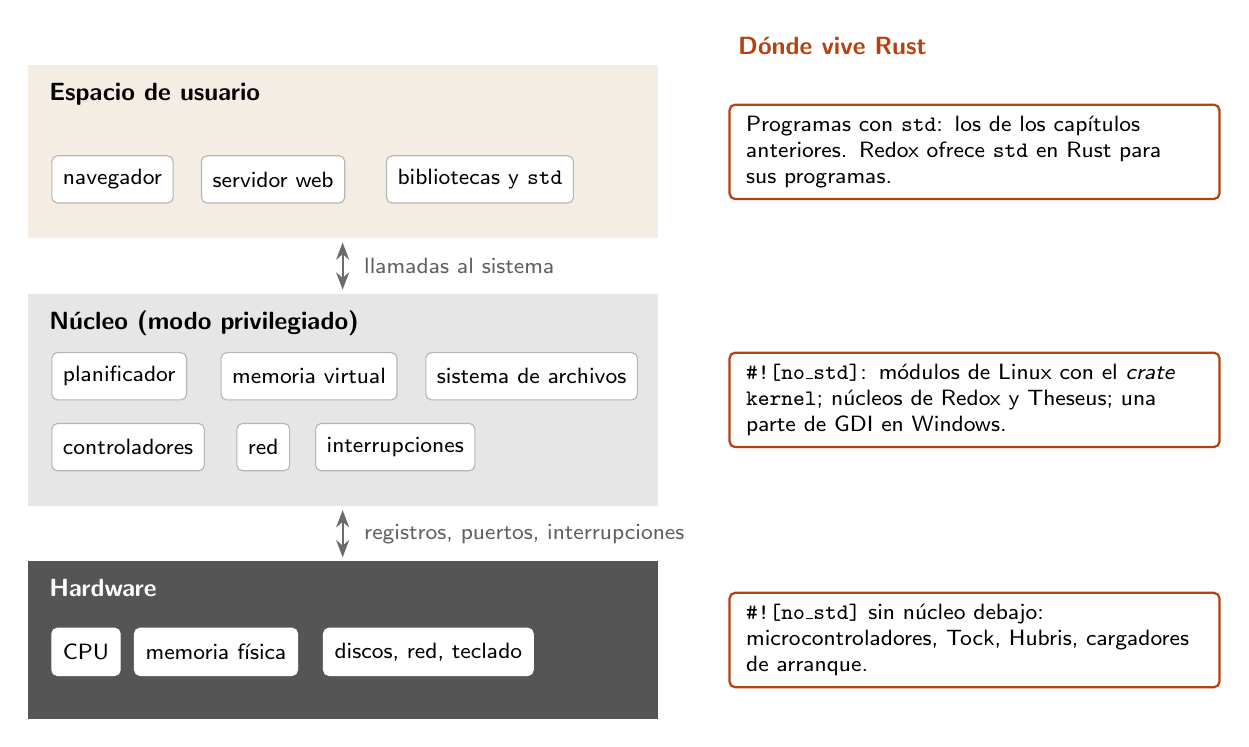
\begin{tikzpicture}[>={Stealth[length=2.2mm]},
  execute at begin node={\hyphenpenalty=10000},
  capa/.style={draw=none,minimum width=78mm,minimum height=17mm,
    anchor=north west,inner sep=0pt},
  pieza/.style={draw=carbon!35,fill=white,rounded corners=2pt,
    font=\sffamily\footnotesize,inner xsep=4pt,inner ysep=3pt,
    minimum height=6mm},
  rust/.style={draw=oxido,line width=0.8pt,fill=white,
    font=\sffamily\footnotesize,text width=58mm,align=left,
    inner xsep=6pt,inner ysep=4pt,anchor=west,rounded corners=2pt},
  rot/.style={font=\sffamily\small\bfseries,anchor=north west},
  nota/.style={font=\sffamily\footnotesize,text=carbon!75}]
  % Capas
  \fill[arena] (0,0) rectangle (8,-2.2);
  \fill[carbon!12] (0,-2.9) rectangle (8,-5.6);
  \fill[carbon!80] (0,-6.3) rectangle (8,-8.3);
  \node[rot] at (0.15,-0.1) {Espacio de usuario};
  \node[rot] at (0.15,-3.0) {Núcleo (modo privilegiado)};
  \node[rot,text=white] at (0.15,-6.4) {Hardware};
  % Piezas
  \node[pieza,anchor=west] at (0.3,-1.45) {navegador};
  \node[pieza,anchor=west] at (2.2,-1.45) {servidor web};
  \node[pieza,anchor=west] at (4.55,-1.45) {bibliotecas y \texttt{std}};
  \node[pieza,anchor=west] at (0.3,-3.95) {planificador};
  \node[pieza,anchor=west] at (2.45,-3.95) {memoria virtual};
  \node[pieza,anchor=west] at (5.05,-3.95) {sistema de archivos};
  \node[pieza,anchor=west] at (0.3,-4.85) {controladores};
  \node[pieza,anchor=west] at (2.65,-4.85) {red};
  \node[pieza,anchor=west] at (3.65,-4.85) {interrupciones};
  \node[pieza,anchor=west,draw=white] at (0.3,-7.45) {CPU};
  \node[pieza,anchor=west,draw=white] at (1.35,-7.45) {memoria física};
  \node[pieza,anchor=west,draw=white] at (3.75,-7.45) {discos, red, teclado};
  % Fronteras
  \draw[<->,carbon!70,thick] (4,-2.25) -- (4,-2.85);
  \node[nota,anchor=west] at (4.15,-2.55) {llamadas al sistema};
  \draw[<->,carbon!70,thick] (4,-5.65) -- (4,-6.25);
  \node[nota,anchor=west] at (4.15,-5.95) {registros, puertos, interrupciones};
  % Dónde vive Rust
  \node[font=\sffamily\small\bfseries,text=oxido,anchor=west] at (8.9,0.25) {Dónde vive Rust};
  \node[rust] at (8.9,-1.1) {Programas con \texttt{std}: los de los capítulos anteriores. Redox ofrece \texttt{std} en Rust para sus programas.};
  \node[rust] at (8.9,-4.25) {\texttt{\#![no\_std]}: módulos de Linux con el \emph{crate} \texttt{kernel}; núcleos de Redox y Theseus; una parte de GDI en Windows.};
  \node[rust] at (8.9,-7.3) {\texttt{\#![no\_std]} sin núcleo debajo: microcontroladores, Tock, Hubris, cargadores de arranque.};
\end{tikzpicture}
\end{document}
